%!TEX encoding = UTC-8 Unicode
\documentclass[submission, Phys, hidelnks]{SciPost}
\usepackage{braket}
\usepackage[ruled, vlined]{algorithm2e}
\usepackage{amsmath, bm}
\usepackage{dsfont}
\usepackage{listings}
\usepackage{color}
\usepackage{xcolor}
\DeclareFixedFont{\ttb}{T1}{txtt}{bx}{n}{10}
\DeclareFixedFont{\ttm}{T1}{txtt}{m}{n}{10}
\definecolor{deepblue}{rgb}{0,0,0.7}
\definecolor{deepred}{rgb}{0.6,0,0}
\definecolor{deepgreen}{rgb}{0,0.5,0}
\newcommand\pythonstyle{\lstset{
    language=Python,
    keepspaces=true, 
    basicstyle=\ttfamily\footnotesize,
    tabsize=3,
    keywordstyle=\color{keywordcolour},
    %otherkeywords={self}, 
    frame = single,
    keywordstyle=\ttb\color{deepblue},
    emph={qucumber, state, SigmaX, SigmaZ, __init__},
    emphstyle=\color{deepred},
    stringstyle=\color{deepgreen},
    showstringspaces=false,
    commentstyle  = \color{deepgreen}\ttfamily
}}
\lstnewenvironment{python}[1][]{
    \pythonstyle
    \lstset{#1}
}
{}
\newcommand\pythoninline[1]{{\pythonstyle\lstinline!#1!}}
\newcommand{\red}[1]{{\color{red} #1}}
\SetKwComment{Comment}{$\triangleright$\ }{}

\begin{document}

\begin{center}{\Large \textbf{
    QuCumber: wavefunction reconstruction with neural networks
}}\end{center}

\begin{center}
    Matthew J.~S.~Beach\textsuperscript{1,2},
    Isaac De Vlugt\textsuperscript{1},
    Anna Golubeva\textsuperscript{1,2},
    Patrick Huembeli\textsuperscript{2,3},
    Roger G.~Melko\textsuperscript{1,2*},
    Ejaaz Merali\textsuperscript{1},
    Giacomo Torlai\textsuperscript{1,2},
\end{center}

\begin{center}
    {\bf 1} 
    Department of Physics and Astronomy, University of Waterloo,
    Ontario N2L 3G1, Canada
    \\
    {\bf 2} Perimeter Institute for Theoretical Physics, Waterloo,
    Ontario N2L 2Y5, Canada
    \\
    {\bf 3} ICFO-Institut de Ciencies Fotoniques, Barcelona Institute of Science and Technology,
    08860 Castelldefels (Barcelona), Spain\\

    * \href{mailto:rgmelko@uwaterloo.ca}{rgmelko@uwaterloo.ca} \\
\end{center}

\begin{center}
    \today
\end{center}

%\linenumbers

\section*{Abstract}
{\bf
    \red{
        In this post, we present QuCumber, an open-source Python package that implements restricted Boltzmann machines to reconstruct unknown quantum states from experimental measurements. The effectiveness of modern machine learning algorithms in compressing high-dimensional data allows neural networks to discover compact representations of a quantum state, and reconstruct traditionally challenging physical properties, not directly accessible in current experiments. We show how to use QuCumber to reconstruct wavefunctions with and without a phase structure and deploy the trained network to estimate expectation values of various physical observables.
    }
}

\vspace{10pt}
\noindent\rule{\textwidth}{1pt}
\tableofcontents\thispagestyle{fancy}
\noindent\rule{\textwidth}{1pt}
\vspace{10pt}

\section{Introduction}
The current advances in designing and building quantum technologies, as well as in the reliable control of synthetic quantum matter, is leading to a new wave of quantum hardware, where highly pure quantum states are routinely prepared in laboratories. Notwithstanding the presence of noise and decoherence, new exciting possibilities have been recently opened by this class of ``noisy" quantum hardware. Notable examples are the quantum-assisted simulation of small molecules and quantum magnets with superconducting hardware~\cite{gambetta17,gambetta18}, and the preparation of ground states breaking different spacial symmetries using a cold Rydberg atom quantum simulator~\cite{Bernien17}. As this generation of quantum technologies grow, the number of quantum degrees of freedom (e.g.~qubits, atoms, etc.), reliable and scalable classical algorithms are required to aid in the analysis and verification of the quantum devices. This is necessary to extract physical observables otherwise inaccessible from experimental measurements, as well as identifying the source of noise to provide direct feedback for improving the hardware quality. Traditional approaches for reconstructing unknown quantum states from a set of measurements -- quantum state reconstruction (QSR) -- suffer the exponential overhead that is typical of quantum many-body systems and thus remain suited for systems with a small number of constituents. 

Recently, an alternative path to QSR was put forward, based on modern machine learning (ML) techniques~\cite{torlai2018tomography, TorlaiMixed}. This approach relies on a powerful generative model called a {\it restricted Boltzmann machine} (RBM)~\cite{Smolensky}, a stochastic neural network with two layers of binary units. The visible layer $\bm{\mathrm{x}}=(\mathrm{x}_1,\dots,\mathrm{x}_N)$ describes the physical degrees of freedom, and a hidden layer $\bm{\mathrm{h}}=(\mathrm{h}_1,\dots,\mathrm{h}_{N_h})$, used to capture high-order correlation between the visible units. Given the set of neural network parameters $\bm{\lambda}$, the RBM defines a probabilistic model described by the parametric distribution $p_{\bm{\lambda}}(\bm{\mathrm{x}})$ (see Glossary). RBMs have been widely used in the ML community for the pre-training of deep neural networks~\cite{Hinton06} and compressing high-dimensional data into lower-dimensional representations~\cite{Hinton504}. More recently, RBMs have been adopted by the physics community in the context of representing both classical and quantum many-body states~\cite{Torlai2016thermo, CarleoTroyer2017Science}, and are currently being investigated in the context of their representational power, their connection with tensor network states~\cite{GlasserCirac2018} and the renormalization group~\cite{Maciej}.

In this post, we present QuCumber, a {\it quantum calculator used for many-body eigenstates reconstruction}. QuCumber is an open-source Python package that implements the neural-network QSR of many-body wavefunctions from measurement data, directly accessible in most experimental setups. Some examples are magnetic spin projections, orbital occupation number, and the logical state of qubits. Given a training dataset of measurements, QuCumber discovers the most likely quantum state compatible with the measurements by finding the optimal set of parameters $\bm{\lambda}$ of an RBM. A properly trained RBM is an approximation of the unknown quantum state underlying the data and can be used to calculate various physical observables of interest, such as entanglement entropy~\cite{torlai2018tomography}.

In Section \ref{sec:positive}, we introduce the reconstruction technique for the case of positive wavefunctions where all coefficients are (or can be transformed to be) real and positive. We discuss the required format for input data, as well as training of the RBM and the reconstruction of both diagonal and off-diagonal observables using a trained RBM. In Section~\ref{sec:complex}, we consider the more general case of a complex-valued wavefunction. We show the general strategy to extract the phase structure from raw data by performing appropriate unitary rotations on the state before measurements. We then show a practical reconstruction of an entangled state of two qubits. A glossary of useful terms and equations can be found at the end of the post in Section~\ref{Glossary}.

\section{Positive wavefunctions}\label{sec:positive}
In this Section, we present the application of QuCumber to reconstruct many-body quantum states described by wavefunctions $|\Psi\rangle$ with positive coefficients $\Psi(\bm{\mathrm{x}})=\langle\bm{\mathrm{x}}|\Psi\rangle \ge0$, where $|\bm{\mathrm{x}}\rangle=|\mathrm{x}_1,\dots,\mathrm{x}_N\rangle$ is a reference basis for the Hilbert space of $N$ quantum degrees of freedom. The neural-network QSR requires raw data $\mathcal{D}=(\bm{\mathrm{x}}_1,\bm{\mathrm{x}}_2,\dots)$ generated through projective measurements of the state $|\Psi\rangle$ in the reference basis. These measurements adhere to the probability distribution given by the Born rule, $P(\bm{\mathrm{x}})=|\Psi(\bm{\mathrm{x}})|^2$. Since the wavefunction is strictly positive, the quantum state is completely characterized by the measurement distribution, $\Psi(\bm{\mathrm{x}})=\sqrt{P(\bm{\mathrm{x}})}$. 

The positivity of the wavefunction allows a simple and natural connection between quantum states and classical probabilistic models. Specifically, QuCumber employs the probability distribution $p_{\bm{\lambda}}(\bm{\mathrm{x}})$ of an RBM to capture the distribution $P(\bm{\mathrm{x}})$ underlying the measurement data. Using contrastive divergence (CD)~\cite{hinton2002training}, QuCumber trains the RBM to discover a set of parameters $\bm{\lambda}^*$ that minimize the Kullback-Leibler (KL) divergence between the two distributions. Upon successful training ($p_{\bm{\lambda}^*}(\bm{\mathrm{x}})\sim P(\bm{\mathrm{x}})$), we obtain a faithful representation of the target quantum state,
\begin{equation}\label{wfpd}
    \psi_{\bm{\lambda}^*}(\bm{\mathrm{x}})= \sqrt{p_{\bm{\lambda}^*}(\bm{\mathrm{x}})}
    \simeq\Psi(\bm{\mathrm{x}})\:.
\end{equation} 

In the following Sections, we present a demonstration of reconstructing the ground-state wavefunction of the one-dimensional transverse-field Ising model (TFIM) with QuCumber. We take Hamiltonian
\begin{equation}
    \hat{H} = -J\sum_i \hat{\sigma}^z_i \hat{\sigma}^z_{i+1} - h \sum_i\hat{\sigma}^x_i\:, \label{TFIM}
\end{equation}
where $\sigma^{x/z}_i$ are spin-1/2 Pauli matrices on site $i$ and we assume open boundary conditions. For this example, we consider a chain with $N=10$ spins at the quantum critical point $J=h=1$.

\subsection{Setup}\label{subsec:example}
Rather than experimental data, we use a set of projective measurements generated withsampling from the exact ground-state wavefunction. Given the small size of the system, the ground state, $|\Psi\rangle$, can be found with exact diagonalization. The training dataset, $\mathcal{D}$, is generated by sampling the distribution $P(\bm{\sigma}^z)=|\Psi(\bm{\sigma}^z)|^2$, obtaining a sequence of $N_S=10^5$ independent spin projections in the $\bm{\sigma}^z$ basis
\footnote{The training dataset can be download from
    \href{https://github.com/PIQuIL/QuCumber/blob/master/examples/Tutorial1_TrainPosRealWavefunction/tfim1d_data.txt}{\texttt{https://github.com/PIQuIL/QuCumber/blob/master/\\examples/Tutorial1\_TrainPosRealWavefunction/tfim1d\_data}}
}
Each data point in $\mathcal{D}$ consists of an array $\bm{\sigma}^z_j=(\sigma^z_1,\dots,\sigma^z_N)$ with shape \verb|(N,)| and should be passed to QuCumber as a numpy array or torch tensor. For example, $\bm{\sigma}^z_j=$ \verb|np.array([1,0,1,1,0,1,0,0,0,1])|, where we use $\sigma_j^z=0,1$ to represent a spin-down and spin-up state respectively. Therefore, the entire input data set is contained into an array with shape \verb|(N_S, N)|.

Aside from the training data, QuCumber also allows us to import an example wavefunction. This can be useful for monitoring the quality of the reconstruction during training. In our case, we import the exact ground state to evaluate the fidelity between the QSR $\psi_{\bm{\lambda}^*}(\bf{x})$ and the exact wavefunction $\Psi(\bm{x})$.
The training dataset, \verb|train_data|, and the exact ground state, \verb|true_psi|, are loaded with the data loading utility as follows:
\begin{python}
import qucumber.utils.data as data
train_path = "tfim1d_data.txt"
psi_path = "tfim1d_psi.txt"
train_data, true_psi = data.load_data(train_path, psi_path)
\end{python}
If \verb|psi_path| is not provided, QuCumber will load only the training data. 

Next, we initialize an RBM quantum state $\psi_{\bm{\lambda}}(\bm{\sigma}^z)$ with random weights and zero biases using the constructor \verb|PositiveWavefunction|
\begin{python}
from qucumber.nn_states import PositiveWavefunction
state = PositiveWavefunction(num_visible=10, num_hidden=10)
\end{python}
The number of visible units (\verb|num_visible|) must be equal to the number $N$ of spins, while the number of hidden units (\verb|num_hidden|) can be adjusted to systematically increase the representational power of the RBM. 

The quality of the reconstruction will depend on the specific wavefunction and the ratio of visible to hidden units, $\alpha = \verb|num_hidden|/\verb|num_visible|$.
In practice, we find that $\alpha = 1$ typically leads to good approximations of positive wavefunctions~\cite{Torlai2016thermo}. However, in the general case, the value of $\alpha$ required for a given wavefunction reconstruction should be explored and adjusted by the user.


\subsection{Training}
Once an appropriate representation of the quantum state has been defined, QuCumber trains the RBM through the function \verb|PositiveWavefunction.fit|. Several input parameters need to be provided aside from the training dataset (\verb|train_data|). These include the number of training iterations (\verb|epochs|), the number of samples used for the positive/negative phase of CD (\verb|pos_batch_size|/\verb|neg_batch_size|), the learning rate (\verb|lr|) and the number of sampling steps in the negative phase of CD (\verb|k|). The last argument (\verb|callbacks|) allows the user to pass a set of functions to be evaluated during training.

As an example of a callback, we show the \verb|MetricEvaluator|, which evaluates a function \verb|log_every| epochs during training. Given the small system size and the knowledge of the true ground state, we can evaluate the fidelity between the RBM state and the true ground-state wavefunction (\verb|true_psi|). Similarly, we can calculate the KL divergence between the RBM distribution $p_{\bm{\lambda}}(\bm{x})$, and the data distribution $P(\bm{x})$, which should approach zero for a properly trained RBM. For the current example, we monitor the fidelity and KL divergence (defined in \verb|qucumber.utils.training_statistics|):
\begin{python}
from qucumber.callbacks import MetricEvaluator
import qucumber.utils.training_statistics as ts
log_every = 10
space = state.generate_hilbert_space(10)
callbacks = [
    MetricEvaluator(
        log_every,
        {"Fidelity": ts.fidelity, "KL": ts.KL},
    target_psi=true_psi,
    space=space,
    verbose=True
    )
]
\end{python}
With \verb|verbose=True|, the program will print the epoch number and all callbacks every \verb|log_every| epochs. Now that the metrics to monitor during training have been chosen, we can invoke the optimization with the \verb|fit| function of \verb|PositiveWavefunction|.
\begin{python}
state.fit(
    train_data,
    epochs=400,
    pos_batch_size=100
    neg_batch_size=100,
    lr=0.01
    k=5,
    callbacks=callbacks,
)
\end{python}

Figure \ref{fig:KL} shows the convergence of the fidelity and KL divergence during training. The convergence time will, in general, depend on the choice of hyperparameters.

The network parameters $\bm{\lambda}$, together with the callbacks, can be saved (or loaded) to a file:
\begin{python}
state.save(
    "filename.pt",
    metadata={
        "fidelity": callbacks[0].Fidelity,
        "KL": callbacks[0].KL
    },
)
state.load("filename.pt")
\end{python}

\begin{figure}[hbt]
    \centering{}
    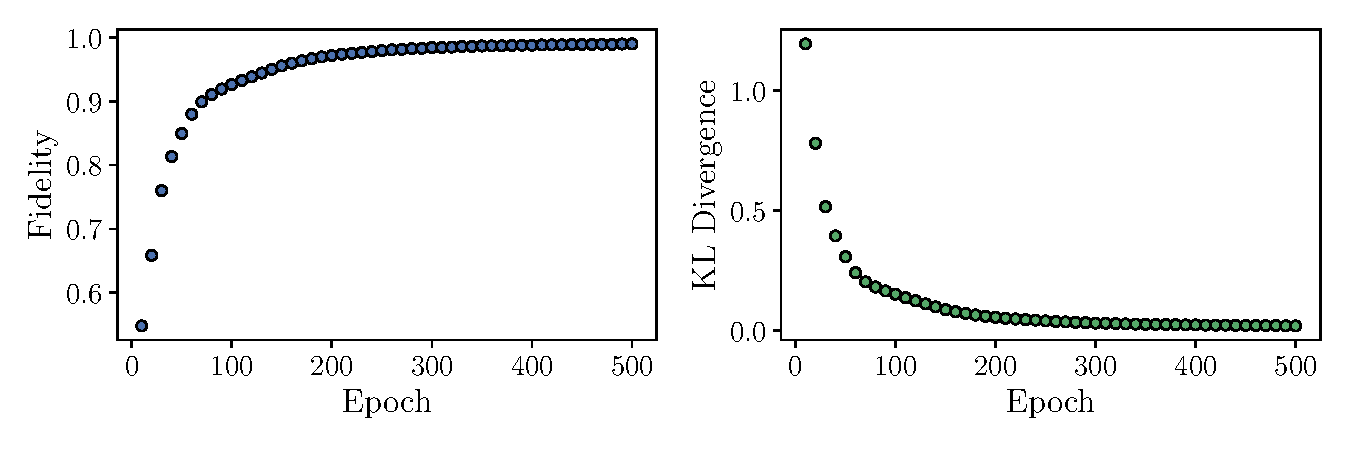
\includegraphics[width=\textwidth]{fid_KL.pdf}
    \caption{\label{fig:KL} The fidelity (left) and the KL divergence (right) during training for the reconstruction of the ground state of the one-dimensional TFIM.}
\end{figure}

In this Section, we demonstrated to most basic aspects of QuCumber regarding training a model and verifying its accuracy. While this example relied on a small data set of $N=10$ spins, QuCumber is not limited to small systems. For a system with an unknown ground state, it is impossible to compute the fidelity as a signal of convergence. Instead, users should rely on other physical observables like the energy. In the following Section, we show how to compute diagonal and off-diagonal observables in QuCumber. 

\subsection{Reconstruction of physical observables} \label{Sec:Sampling_a-Trained_RBM}
In this Section, we discuss how to calculate the average value of a generic physical observable $\hat{\mathcal{O}}$ from a trained RBM. We start with the case of observables that are diagonal in the reference basis in which the RBM was trained. We then show the more general case of off-diagonal observables.

\subsubsection{Diagonal observables}
We begin by considering an observable with only diagonal matrix elements,
$\langle\bm{\sigma}|\hat{\mathcal{O}}|\bm{\sigma}^{\prime}\rangle=\mathcal{O}_{\bm{\sigma}}\delta_{\bm{\sigma\sigma}^\prime}$ where for convenience we take $\bm{\sigma}=\bm{\sigma}^z$ unless otherwise stated.
The expectation value of $\hat{\mathcal{O}}$ is given by
\begin{equation}
    \langle \hat{\mathcal{O}} \rangle = \frac{1}{\sum_{\bm{\sigma}} |\psi_{\bm{\lambda}}(\bm{\sigma})|^2}
    \sum_{\bm{\sigma}} \mathcal{O}_{\bm{\sigma}}|\psi_{\bm{\lambda}}(\bm{\sigma})|^2\:.
\end{equation}
In this case, the exponential sum can be approximated by a Monte Carlo average
\begin{equation}
    \langle \hat{\mathcal{O}}\rangle \approx \frac{1}{N_{\rm MC}} \sum_{k=1}^{N_{\rm MC}} \mathcal{O}_{\bm{\sigma}_k}\:,
\end{equation}
where the spin configurations $\bm{\sigma}_k$ are sampled from the RBM distribution $p_{\bm{\lambda}}(\bm{\sigma})$. This process is particularly efficient given the bipartite structure of the network which allows the use of block Gibbs sampling. 


A simple example for the TFIM is the average magnetization per spin, $M=\sum_j\langle\hat{\sigma}_j\rangle/N$, which can be calculated directly on the spin configuration sampled by the RBM (i.e.,~the state of the visible layer). The visible samples are obtained with the \verb|sample| function of the RBM state object:
\begin{python}
samples = state.sample(num_samples=1000, k=10)
\end{python}
which inputs the total number of samples (\verb|num_samples|) and the number of iterations (\verb|k|) of a block Gibbs step. Once these samples are obtained, the magnetization can be calculated simply as
\begin{python}
magnetization = samples.mul(2.0).sub(1.0).mean(1).abs().mean()
\end{python}
where we converted the binary samples of the RBM back into $\pm 1$ spins.

\subsubsection{Off-diagonal observables}
We turn now to the case of off-diagonal observables, where the expectation value now takes the following form
\begin{equation}
    \langle \hat{\mathcal{O}} \rangle = \frac{1}{\sum_{\bm{\sigma}} |\psi_{\bm{\lambda}}(\bm{\sigma})|^2}
    \sum_{\bm{\sigma\sigma}^\prime} \psi_{\bm{\lambda}}(\bm{\sigma})
    \psi_{\bm{\lambda}}(\bm{\sigma}^\prime)\mathcal{O}_{\bm{\sigma\sigma}^\prime}\:.
\end{equation}
This expression can once again be approximated with a Monte Carlo average 
\begin{equation}
    \langle \hat{\mathcal{O}}\rangle \approx \frac{1}{N_{\rm MC}} \sum_{k=1}^{N_{\rm MC}} \mathcal{O}^{[L]}_{\bm{\sigma}_k}
\end{equation}
of the so-called \emph{local estimate} of the observable: 
\begin{equation}
    \mathcal{O}^{[L]}_{\bm{\sigma}_k}=\sum_{\bm{\sigma}^\prime}\frac{\psi_{\bm{\lambda}}(\bm{\sigma}^\prime)}{\psi_{\bm{\lambda}}(\bm{\sigma})} \mathcal{O}_{\bm{\sigma\sigma}^\prime}\:.
\end{equation}
As long as the matrix representation $\mathcal{O}_{\bm{\sigma\sigma}^\prime}$ is sufficiently sparse in the reference basis, the summation can be evaluated efficiently. As an example, we consider the specific case of the transverse magnetization for the $j$-th spin, $M_j^x=\langle\hat{\sigma}^x_j\rangle$, with matrix elements
\begin{equation}
    \langle\bm{\sigma}|\hat{\sigma}^x_j|\bm{\sigma}^{\prime}\rangle=\delta_{\sigma_j^\prime,1-\sigma_j}\prod_{i\ne j}\delta_{\sigma_i^\prime,\sigma_j}\:.
\end{equation}
Therefore, the expectation values reduces to the Monte Carlo average of the local observable
\begin{equation}
    {M_j^x}^{[L]}=\frac{\psi_{\bm{\lambda}}(\sigma_1,\dots,1-\sigma_j,\dots,\sigma_N)}
    {\psi_{\bm{\lambda}}(\sigma_1,\dots,\sigma_j,\dots,\sigma_N)} 
\:.
\end{equation}
evaluated on spin configurations $\bm{\sigma}_k$ sampled from the RBM distribution $p_{\bm{\lambda}}(\bm{\sigma})$. 

QuCumber provides an interface for sampling off-diagonal observables in the \verb|Observable| class. Thorough examples can are available in the tutorial section in the \href{https://qucumber.readthedocs.io/en/stable/}{documentation}\!\!
\footnote{The observables tutorial can be found at 
    \href{https://qucumber.readthedocs.io/en/stable/\_examples/Tutorial3\_DataGeneration\_CalculateObservables/tutorial\_sampling\_observables.html
}{\texttt{https://qucumber.readthedocs.io/en/stable/\_examples\\/Tutorial3\_DataGeneration\_CalculateObservables/tutorial\_sampling\_observables.html}}
}. 
As an example, $\sigma^x$ can be written as an observable class with
\begin{python}
class SigmaX(Observable):

    def apply(self, nn_state, samples):
        psi = nn_state.psi(samples)
        psi_ratio_sum = torch.zeros_like(psi)

        for i in range(samples.shape[-1]):  # sum over spin sites
            flip_spin(i, samples)  # flip the spin at site i
            # compute ratio of psi_(-i) / psi and add it to the running sum
            psi_ratio = nn_state.psi(samples)
            psi_ratio = cplx.elementwise_division(psi_ratio, psi)
            psi_ratio_sum.add_(psi_ratio)
            flip_spin(i, samples)  # flip it back

        # take real part (imaginary part should be approximately zero)
        # and divide by number of spins
        return psi_ratio_sum[0].div_(samples.shape[-1])
\end{python}
%class SigmaZ(Observable):
    %def __init__(self):
        %super(SigmaZ, self).__init__()

    %def apply(self, state, samples):
        %sigma_z = samples.mul(2.).sub(1.).mean(1).abs()
        %return sigma_z
The value of the observable is computed with 
\begin{python}
SigmaX.statistics_from_samples(state, samples)
\end{python}
Similarly, the user can define other observables like $\sigma^z$ or the energy. 

The reconstruction of two magnetic observables for the TFIM is shown in Fig.~\ref{tfim_magn}, where a different RBM was trained for each value of the transverse field $h$. In the left plot, we show the average longitudinal magnetization per site, which can be calculated directly from the configurations sampled by the RBM. In the right plot, we show the off-diagonal observable of transverse magnetization. In both cases, QuCumber successfully discovers a set of parameters $\bm{\lambda}^*$ that correctly approximates the ground-state wavefunction underlying the data.

\begin{figure}[htb]
    \centering{}
    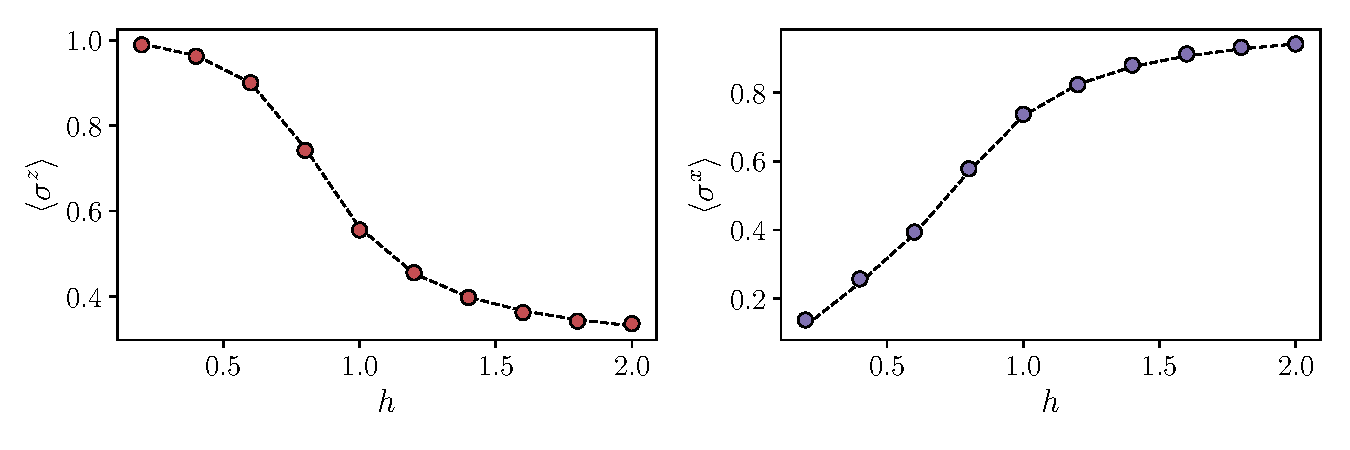
\includegraphics[width=\columnwidth]{obs.pdf}
    \caption{\label{tfim_magn} Reconstruction of the magnetic observables for the TFIM chain with $N=10$ spins. We show the average longitudinal (left) and transverse (right) magnetization per site obtained by sampling a trained RBM. The dashed line denotes the results from exact diagonalization.}
\end{figure}


\section{Complex wavefunctions}
\label{sec:complex}
For positive wavefunctions, the probability distribution underlying the outcomes of projective measurement in the reference basis already contains all the information about the unknown quantum state. In this Section, we consider a target quantum state with a non-trivial sign/phase structure. This means that the wavefunction coefficients in the reference basis can be of different signs, as well as complex-valued, $\Psi(\bm{\sigma})=\Phi(\bm{\sigma})e^{i\theta(\bm{\sigma})}$. We first need to generalize the RBM representation of the quantum state to capture generic complex wavefunctions. To this end, we introduce an additional RBM with network parameters $\bm{\mu}$ and define the total RBM state as:
\begin{equation}
    \psi_{\bm{\lambda} \bm{\mu}} (\bm{\sigma})= \sqrt{p_{\bm{\lambda}} (\bm{\sigma})} e^{i \phi_{\bm{\mu}} (\bm{\sigma})/2}
\end{equation}
where we choose $\phi_{\bm{\mu}}(\bm{\sigma}) = \log (p_{\bm{\mu}} (\bm{\sigma}))$ \cite{torlai2018tomography}. Furthermore, the reconstruction requires a different type of measurement settings. In fact, projective measurements in the reference basis do not convey any information on the phases $\theta(\bm{\sigma})$, since $P(\bm{\sigma})=|\Psi(\bm{\sigma})|^2=\Phi^2(\bm{\sigma})$.

\begin{figure}[htb]
    \centering
    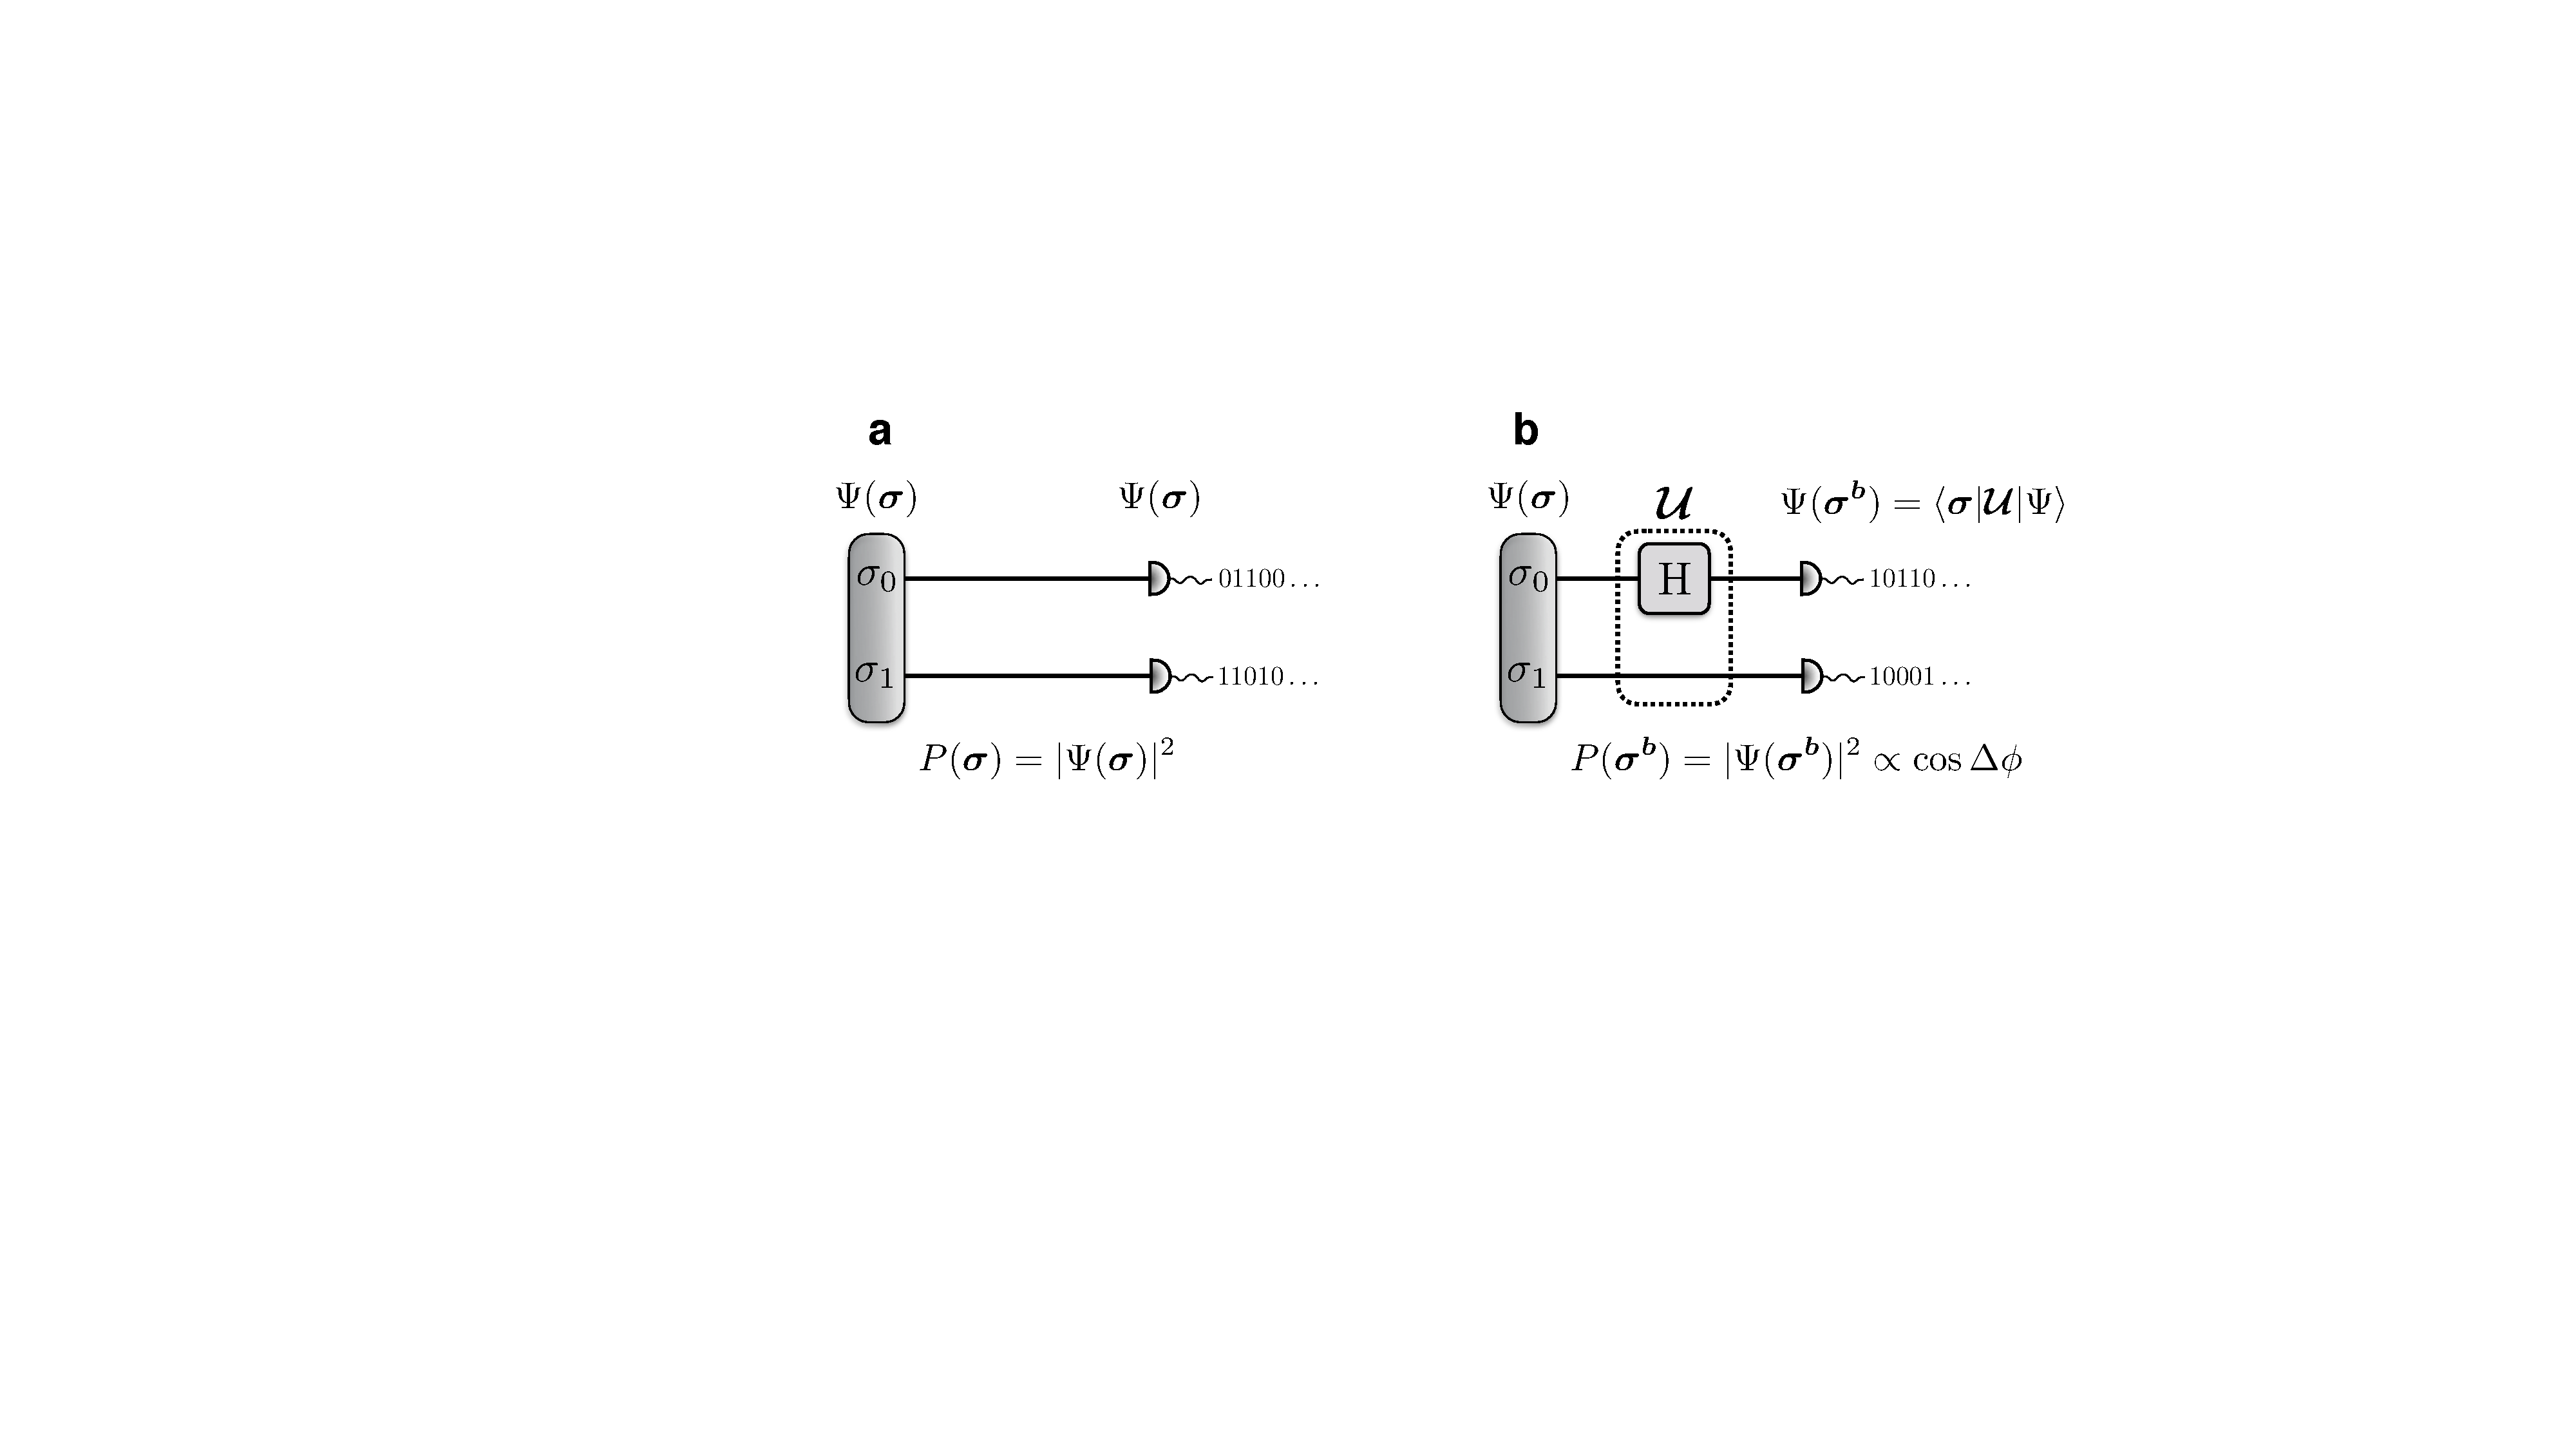
\includegraphics[width=\columnwidth, trim={0 0 0 40}, clip]{2qubits_rotation}
    \caption{Unitary rotations for two qubits. (left) Measurements on the reference basis. (right) Measurement in the rotated basis. The unitary rotation (the Hadamard gate on qubit $\sigma_0$) is applied after state preparation and before the projective measurement.}
    \label{phase_learn} 
\end{figure}

The general strategy to learn a phase structure is to apply a unitary transformation $\bm{\mathcal{U}}$ to the state $|\Psi\rangle$ (before the measurements) such that the resulting measurement distribution $P^{\:\prime}(\bm{\sigma})=|\Psi^\prime(\bm{\sigma})|^2$ of the rotated state $\Psi^\prime(\bm{\sigma})=\langle\bm{\sigma}|\:\bm{\mathcal{U}}\:|\Psi\rangle$ contains fingerprints of the phases $\theta(\bm{\sigma})$ (Fig.~\ref{phase_learn}). In general, different rotations must be independently applied to gain full information on the phase structure. We make the assumption of a tensor product structure of the rotations, $\bm{\mathcal{U}}=\bigotimes_{j=1}^N\hat{\mathcal{U}}_j$. This is equivalent to a local change of basis from $|\bm{\sigma}\rangle$ to $\{|\bm{\sigma}^{\bm{b}}\rangle=|\sigma_1^{b_1},\dots,\sigma_N^{b_N}\rangle\}$, where the vector $\bm{b}$ identifies the local basis $b_j$ for each site $j$. The target wavefunction in the new basis is given by
\begin{equation}
\begin{split}
    \Psi(\bm{\sigma}^{\bm{b}})
    &=\langle \bm{\sigma}^{\bm{b}}|\Psi\rangle=\sum_{\bm{\sigma}}\langle \bm{\sigma}^{\bm{b}}|\bm{\sigma}\rangle\langle\bm{\sigma}|\Psi\rangle\\
    &=\sum_{\bm{\sigma}}\mathcal{U}(\bm{\sigma}^{\bm{b}},\bm{\sigma})\Psi(\bm{\sigma})\:,
\end{split}
\end{equation}
and the resulting measurement distribution is
\begin{equation}
    P_{\bm{b}}(\bm{\sigma}^{\bm{b}})=\bigg|\sum_{\bm{\sigma}}\mathcal{U}(\bm{\sigma}^{\bm{b}},\bm{\sigma})\Psi(\bm{\sigma})\bigg|^2\:.
\end{equation}
To clarify the procedure, let us consider the simple example of a quantum state of two qubits:
\begin{equation}
    |\Psi\rangle=\sum_{\sigma_0,\sigma_1}\Phi_{\sigma_0\sigma_1}e^{i\theta_{\sigma_0\sigma_1}}|\sigma_0\sigma_1\rangle\:,
\end{equation}
and rotation $\bm{\mathcal{U}}=\hat{\mathrm{H}}_0\otimes\hat{\mathcal{I}}_1$, where $\hat{\mathcal{I}}$ is the identity operator and 
\begin{equation}
    \hat{\mathrm{H}}=\frac{1}{\sqrt{2}}\begin{bmatrix}1 & 1\\
1 & -1
\end{bmatrix}
\end{equation}
is called the {\it Hadamard gate}. This transformation is equivalent to rotating the qubit $\sigma_0$ from the reference ($\sigma_0^z$) basis the the $\sigma_0^x$ basis. A straightforward calculation leads to the following probability distribution of the projective measurement in the new basis $|\sigma_0^x,\sigma_1\rangle$: 
\begin{equation}
    P_{\bm{b}}(\sigma_0^x,\sigma_1)=\frac{\Phi_{0\sigma_1}^2+\Phi_{1\sigma_1}^2}{4}+\frac{1-2\sigma_0^x}{2}\Phi_{0\sigma_1}\Phi_{1\sigma_1}\cos(\Delta\theta)\:,
\end{equation}
where $\Delta\theta=\theta_{0\sigma_1}-\theta_{1\sigma_1}$. Therefore, the statistics collected by measuring in this basis implicitly contains partial information on the phases. To obtain the full phases structure, additional transformations are required, one example being the rotation from the reference basis to the $\sigma^y_j$ local basis, realized by
the elementary gate
\begin{equation}
        \hat{\mathrm{K}}_j=\langle\sigma_j^y|\sigma_j^z\rangle=\frac{1}{\sqrt{2}}\begin{bmatrix}1 & -i\\
    1 & i
\end{bmatrix}\:.
\end{equation}


\subsection{Setup}
We now proceed to use QuCumber to reconstruct a complex-valued wavefunction. For simplicity, we restrict ourselves to two qubits and consider the general case of a quantum state with random amplitudes $\Phi_{\sigma_0\sigma_1}$ and random phases $\theta_{\sigma_0\sigma_1}$. This example is available in the online tutorial.
\footnote{The tutorial for complex wavefunction can be found at
    \href{https://qucumber.readthedocs.io/en/stable/\_examples/Tutorial2_TrainComplexWavefunction/tutorial_qubits.html
    }{\texttt{https://qucumber.readthedocs.io/en/\\stable/\_examples/Tutorial2\_TrainComplexWavefunction/tutorial\_qubits.html}}
}
We begin by importing the required packages:

\begin{python}
from qucumber.nn_states import ComplexWavefunction
import qucumber.utils.unitaries as unitaries
import qucumber.utils.cplx as cplx
\end{python}
Since we are dealing with a complex wavefunction, we load the corresponding module 
\verb|ComplexWavefunction| to build the RBM quantum state $\psi_{\bm{\lambda\mu}}(\bm{\sigma})$. Furthermore, the following additional utility modules are required: the \verb|utils.cplx| backend for complex algebra, and the \verb|utils.unitaries| module  which contains a set of elementary local rotations. By default, the set of unitaries include rotation to the $\sigma^x$ and $\sigma^y$ local basis implemented by the $\hat{\mathrm{H}}$ and $\hat{\mathrm{K}}$ gates respectively.

We continue by loading the data in QuCumber, which is done using the \verb|load_data| function of the data utility:
\begin{python}
train_path = "qubits_train.txt"
train_bases_path = "qubits_train_bases.txt"
psi_path = "qubits_psi.txt"
bases_path = "qubits_bases.txt"

train_samples, true_psi, train_bases, bases = data.load_data(
  train_path, psi_path, train_bases_path, bases_path
)
\end{python}
As before, we may load the true target wavefunction from \verb|qubits_psi.txt|, which can be used to calculate the fidelity and KL divergence. In contrast with the positive case, we now have measurements performed in different bases. Therefore, the training data consists of an array of qubits projections $(\sigma_0^{b_0},\sigma_1^{b_1}$) in \verb|qubits_train_samples.txt|, together with the corresponding bases $(b_0,b_1)$ where the measurement was taken, in \verb|qubits_train_bases.txt|. Finally, QuCumber loads the set of all the bases appearing the in training dataset, stored in \verb|qubits_bases.txt|. This is required to properly configure the various elementary unitary rotations that need to be applied to the RBM state during the training. For this example, we generated measurements in the following bases:
\begin{equation}
    (b_0, b_1)=(\mathrm{z},\mathrm{z})\:,\:(\mathrm{x},\mathrm{z})\:,\:(\mathrm{z},\mathrm{x})\:,\:(\mathrm{y},\mathrm{z})\:,\:(\mathrm{z},\mathrm{y})
\end{equation}
Finally, before the training, we initialize the set of unitary rotations and create the RBM state object. In the case of the provided dataset, the unitaries required are the well-known $\hat{\mathrm{H}}$ and $\hat{\mathrm{K}}$ gates. The dictionary needed can be created with \verb|unitaries.create_dict()|. 
By default, when \verb|unitaries.create_dict()| is called, it will contain the identity and the $\hat{\mathrm{H}}$ and $\hat{\mathrm{K}}$ gates with the keys \verb|Z|, \verb|Y|, and \verb|X| respectively. It is possible to add additional gates by specifying them as 
\begin{python}
U = torch.tensor([[re_part], [im_part]], dtype=torch.double)
unitary_dict = unitaries.create_dict(unitary_name="U")
\end{python}
where \verb|re_part|, \verb|im_part|, and \verb|U| are to be specified by the user.

We then initialize the complex RBM object with
\begin{python}
state = ComplexWavefunction(
   num_visible=2 num_hidden=2, unitary_dict=unitary_dict
)
\end{python}

The key difference between positive and complex wavefunction reconstruction is the requirement of additional measurements in different basis. Despite this, loading the data, initializing models, and training the RBMs are all very similar to the positive case.

\subsection{Training}
The training procedure is somewhat similar to the case of a positive wavefunction, where QuCumber optimized the parameters $\bm{\lambda}$ to minimize the KL divergence between the data and the RBM distribution. When measuring in multiple bases, the optimization now runs over the set of parameters $(\bm{\lambda},\bm{\mu})$ and minimizes the sum of KL divergences between the data distribution $P(\bm{\sigma}^{\bm{b}})$ and the RBM distribution $|\psi_{\bm{\lambda\mu}}(\bm{\sigma}^{\bm{b}})|^2$ for each bases $\bm{b}$ appearing in the training dataset. For example, if a given training sample is measured in the basis $(\mathrm{x},\mathrm{z})$, QuCumber applies the appropriate unitary rotation $\bm{\mathcal{U}}=\hat{\mathrm{H}}_0\otimes\hat{\mathcal{I}}_1$ to the RBM state before collecting the gradient signal. 

Similar to the case of positive wavefunction, we generate the Hilbert space (to compute fidelity and KL divergence) and initialize the callbacks
\begin{python}
state.space = nn_state.generate_hilbert_space(nv)
callbacks = [
  MetricEvaluator(
    log_every,
    {"Fidelity": ts.fidelity, "KL": ts.KL},
    target_psi=true_psi,
    bases=bases,
    verbose=True,
    space=state.space,
  )
]

\end{python}
The training is carried out by calling the \verb|fit| function of \verb|ComplexWavefunction|, given the set of hyper-parameters
\begin{python}
state.fit(
    train_samples,
    epochs=200,
    pos_batch_size=10,
    neg_batch_size=10,
    lr=0.05,
    k=5,
    input_bases=train_bases,
    callbacks=callbacks,
)
\end{python}

In Fig.~\ref{fig:complex} we show the total KL divergence and the fidelity with the true two-qubit state during training. 
\begin{figure}[htb]
    \centering{}
    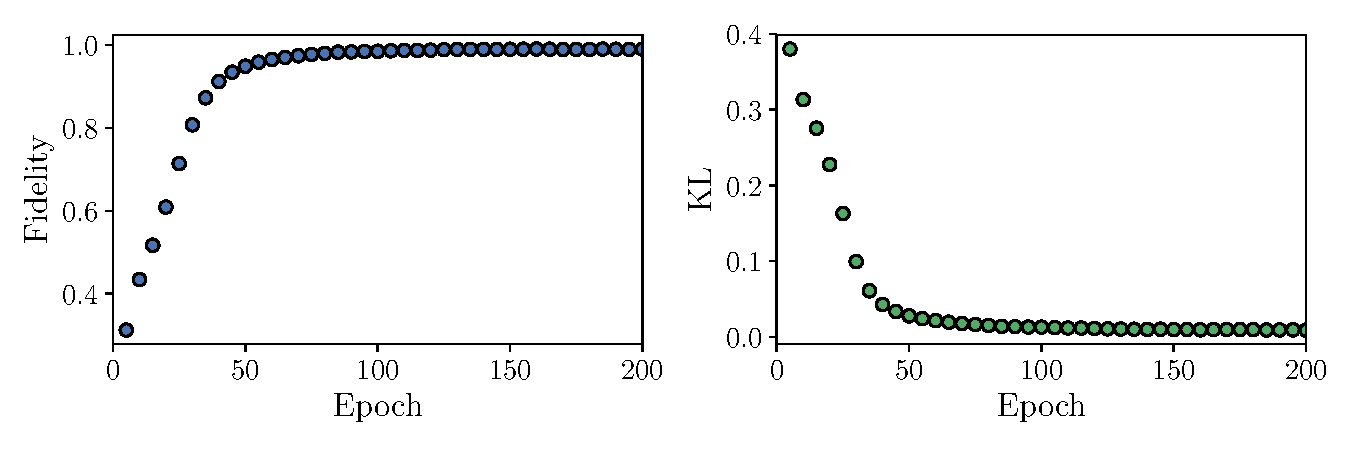
\includegraphics[width=\textwidth]{complex_fid_KL.pdf}
    \caption{\label{fig:complex} Training a complex RBM with QuCumber on random two-qubit data. We show the fidelity (left), and KL divergence (right), as a function of the training epochs.}
\end{figure}

After successfully training a QuCumber model, we can once again compute generic observables in the reference basis.  
\red{[SOMETHING ABOUT OBSERVABLES?!?!?!?!?!??!}
\red{[CONCLUDING PARAGRAPH??]}

\section{Conclusion}
\red{TODO}

\section*{Acknowledgements}
We acknowledge G. Carleo, J. Carrasquilla and L. Hayward Sierens for stimulating discussions. 
We thank J. Matlock and the Perimeter Institute for Theoretical Physics for the continuing support of PIQuIL.

\paragraph{Author contributions}
Authors are listed alphabetically. For an updated record of individual contributions, consult the repository at \url{https://github.com/PIQuIL/QuCumber/graphs/contributors}.

\paragraph{Funding information}

This research was supported by the Natural Sciences and Engineering
Research Council of Canada (NSERC), the
Canada Research Chair program, the Perimeter Institute
for Theoretical Physics, and the National Science Foundation
under Grant No. NSF PHY-1125915. We also gratefully
acknowledge the support of NVIDIA Corporation with
the donation of the Titan Xp GPU used for this research.
Research at Perimeter Institute is supported by the Government
of Canada through Industry Canada and by the
Province of Ontario through the Ministry of Research \&
Innovation. P.~H. acknowledges support from ICFOstepstone, funded by the Marie Sklodowska-Curie Co-funding of regional, national and international programmes (GA665884) of the European Commission, as well as by the Severo Ochoa 2016-2019' program at ICFO (SEV-2015-0522), funded by the Spanish Ministry of Economy, Industry, and Competitiveness (MINECO).


\appendix
\section{Glossary}
\label{Glossary}

We list an overview of terms discussed in the document and relevant for RBMs. For more detail we refer to the code documentation on \url{https://piquil.github.io/QuCumber/}, and References~\cite{hinton2002training, hinton2012practical}.

\begin{itemize}

\item {\it Batch}: The subset of data selected for one iteration of training in stochastic gradient descent.

\item {\it Biases}: For a visible unit $v_j$ and a hidden unit $h_i$, the respective biases in the RBM are $b_j$ and $c_i$. They act like a magnetic field term in the expression for the energy given in Eq.~\eqref{RBMenergy}.

\item {\it Contrastive divergence}: An approximate maximum-likelihood learning algorithm for RBMs \cite{hinton2002training}.

\item {\it Energy}: In analogy to statistical physics, the energy of an RBM is defined given the joint configuration $(v, h)$ of visible and hidden units as follows:
\begin{equation}
   E_{\bm{\lambda}}(v,h) = - \sum\limits_{j=1}^V b_j v_j - \sum\limits_{i=1}^H c_i h_i - \sum\limits_{ij} h_i W_{ij} v_j, \label{RBMenergy}
\end{equation}

\item {\it Effective energy}: Obtained from the energy by tracing out the hidden units $h$; often called the ``free energy'' in machine learning literature.
\begin{equation}
   \mathcal{E}_{\bm{\lambda}}(v) = - \sum\limits_{j=1}^V b_j v_j - \sum\limits_{i=1}^H \log \left\{ 1 + \exp \left( \sum\limits_{j} W_{ij}v_j +c_i\right) \right\}, \label{RBMeffectiveenergy}
\end{equation}

\item {\it Epoch}: A single pass through an entire training set.

\item {\it Hidden units}: There are $H_h$ units in the second layer of the RBM, denoted by the vector $\mathbf{h}=(h_1, ..., h_{zN_h})$, that represent latent variables and are referred to as ``hidden". The number of hidden units can be adjusted to tune the representational capacity of the RBM.

\item{\it Hyperparameter:} The RBM architecture and some parameters of the training procedure that have to be adjusted to achieve effective training. Examples include the learning rate, number of hidden units, batch size, or number of training epochs.

\item {\it Joint distribution}: The RBM assigns a probability to each joint configuration $(v,h)$ according to the Boltzmann distribution:
\begin{equation}
   p_{\bm{\lambda}}(v,h) = \frac{1}{Z_{\bm{\lambda}}} e^{-E_{\bm{\lambda}}(v,h)},
\end{equation}

\item{\it KL divergence}: The Kullback-Leibler divergence, or relative entropy, is a measure for the ``distance" between two probability distributions. The KL divergence of identical distributions is zero, while for orthogonal distributions it is infinite.

\item{\it Learning rate}: A hyperparameter that can be adjusted to affect training performance. Training speed is proportional to the learning rate; however, the chance of finding a suitable minimum of the KL-divergence is higher for low learning rates.

\item {\it Marginal distribution}: Obtained by marginalizing the joint distribution, e.g.
\begin{equation}\label{Eq:marginal_distribution}
   p_{\bm{\lambda}}(v) = \frac{1}{Z_{\bm{\lambda}}} \sum\limits_{h\in \mathcal{H}} e^{-E_{\bm{\lambda}}(v,h)} = \frac{1}{Z_{\bm{\lambda}}} e^{- \mathcal{E}_{\bm{\lambda}}(v)}.
\end{equation}

\item {\it QuCumber}: A quantum calculator used for many-body eigenstate reconstruction.

\item {\it Parameters}: An RBM's energy is defined via a set of neural network parameters $\bm{\lambda} = \{b,c,W\}$, consisting of weights and biases.

\item {\it Partition function}: The normalizing constant of the Boltzmann distribution. It is obtained by summing over all possible pairs of visible and hidden vectors:
\begin{equation}
   Z_{\bm{\lambda}} = \sum\limits_{v\in \mathcal{V}}\sum\limits_{h\in \mathcal{H}} e^{-E_{\bm{\lambda}}(v,h)}.
\end{equation}

\item {\it Restricted Boltzmann Machine}: A two-layer network with bidirectionally connected stochastic processing units. ``Restricted" refers to the connections (or weights) between the visible and hidden units: Each visible unit is connected with each hidden unit, but there are no intra-layer connections.

\item {\it Visible units}: There are $V$ units in the first layer of the RBM, denoted by the vector $v=(v_1, ..., v_V)$, which correspond to the experimental data and are therefore called ``visible". The number of visible units $V$ is fixed to the number of physical qubits.

\item {\it Weights}: $W_{ij}$ is the symmetric connection or interaction between the visible unit $v_j$ and the hidden unit $h_i$.

\end{itemize}


\bibliography{bibliography}
\nolinenumbers
\end{document}

